\begin{figure}[H]
    \centering
    \begin{subfigure}{0.3\textwidth}
        \centering
        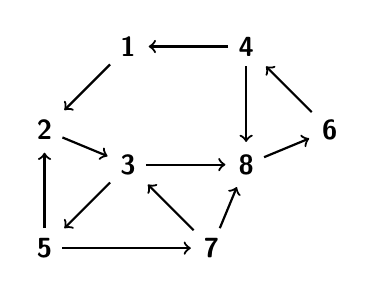
\begin{tikzpicture}[->,shorten >=1pt,auto,node distance=1.5cm,
                            thick,main node/.style={font=\sffamily\bfseries}]

        % Define vertices
        \node[main node] (1) {1};
        \node[main node] (2) [below left of=1] {2};
        \node[main node] (3) [below of=1] {3};
        \node[main node] (4) [right of=1] {4};
        \node[main node] (5) [below left of=3] {5};
        \node[main node] (6) [below right of=4] {6};
        \node[main node] (7) [below right of=3] {7};
        \node[main node] (8) [right of=3] {8};

        % Draw edges
        \path[every node/.style={font=\sffamily\small}]
            (1) edge (2)
            (2) edge (3)
            (3) edge (8)
            (4) edge (1)
            (4) edge (8)
            (5) edge (2)
            (5) edge (7)
            (6) edge (4)
            (7) edge (3)
            (7) edge (8)
            (8) edge (6)
            (3) edge (5);

        \end{tikzpicture}
        \caption{Graph 2}
    \end{subfigure}
    \begin{subfigure}{0.3\textwidth}
        \centering
        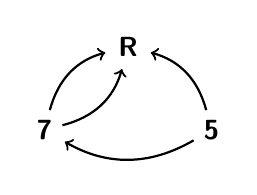
\begin{tikzpicture}[->,shorten >=1pt,auto,node distance=1.5cm,
                            thick,main node/.style={font=\sffamily\bfseries}]

        % Define vertices
        \node[main node] (R) {R};
        \node[main node] (5) [below right of=R] {5};
        \node[main node] (7) [below left of=R] {7};

        % Draw edges
        \path[every node/.style={font=\sffamily\small}]
            (5) edge[bend right] (R)
            (5) edge[bend left] (7)
            (7) edge[bend right] (R)
            (7) edge[bend left] (R);

        \end{tikzpicture}
        \caption{\textsc{Condense}(G) before \textsc{Add}}
        \label{fig:condense_before_add}      
    \end{subfigure}
    \begin{subfigure}{0.3\textwidth}
        \centering
        
\begin{tikzpicture}[->,shorten >=1pt,auto,node distance=1.5cm,
                            thick,main node/.style={draw,circle,font=\sffamily\bfseries}]

        % Define vertices
        \node[main node] (R') {R'};

        \end{tikzpicture}
        \caption{\textsc{Condense}(G) after \textsc{Add}}
        \label{fig:condense_after_add}
    \end{subfigure}
    \caption{Graph 2, \textsc{Condense}(G) before and after \textsc{Add}}
    \label{fig:graph2_condense}
\end{figure}
 